\documentclass{article}
\usepackage{mathtools} % For logical operators
\usepackage{tikz} % For graphs
\usepackage{tgbonum} % For fonts
\usepackage{wasysym} % For symbols

\begin{document}
\section{Exercise 2 - Dans la peau d'Apollon}
We will have to use the following logical predicates:
\begin{itemize}
\item {\fontfamily{qcr}\selectfont
man(person)} - returns TRUE if given person is male, else returns FALSE
\item {\fontfamily{qcr}\selectfont
woman(person)} - returns TRUE if given person is female, else returns FALSE
\item {\fontfamily{qcr}\selectfont
love(person1, person2)} - returns TRUE if person1 loves person2, else returns FALSE. (person1, person2) is an ordered pair, i.e. it may be the case that A loves B and B doesn't love A.
\item {\fontfamily{qcr}\selectfont
couple(person1,person2)} - returns TRUE if person1 is in a relationship with person2, else returns FALSE. (person1, person2) is an unordered pair, i.e. saying that A and B are in a couple is the same thing as saying that B and A are in a couple. 
\end{itemize}
The logical formulae for the given expressions are:
\begin{itemize}

\item \(couple(Alex, Alexandrine) \land couple(Robin, Floriane) \)

\item \( \exists a,b,x,y,m,n: man(a) \land woman(x) \land couple(a,b) \land couple(x,y) \land love(a,b) \land love(x,y) \land love(a,m) \land(x,n) \)

\item \( \exists a,b,x,y , \forall m \neq b,y: man(a) \land woman(x) \land couple(a,b) \land couple(x,y) \land love(a,b) \land love(x,y) \land \neg love(a,m) \land \neg love(x,m) \)

\item \( \exists a,b: love(Miguel,a) \land love(a,b) \land love(b,Alexandrine)\)

\item \( \forall x,y: woman(x) \land love(x,y) \implies man(y) \)

\item \( \exists x,y: love(Robin,x) \land love(x,y) \land love(y,Robin) \)

\item \( \forall x: \neg love(x,x) \)
\end{itemize}

The following graphs satisfies the given constraints:
\\Couple graph
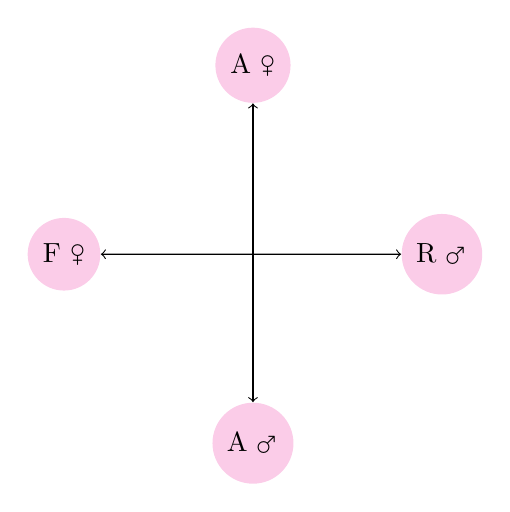
\begin{tikzpicture}
[scale=.8,auto=left,every node/.style={circle,fill=magenta!20}]
\node (Alexandre) at (0,0) {A \mars};
\node (Alexandrine) at (0,6) {A \venus};
\node (Robin) at (3,3) {R \mars};
\node (Floriane) at (-3,3) {F \venus};
\draw[<->] (Alexandre) to (Alexandrine);
\draw[<->] (Robin) to (Floriane);
\end{tikzpicture}

Love graph
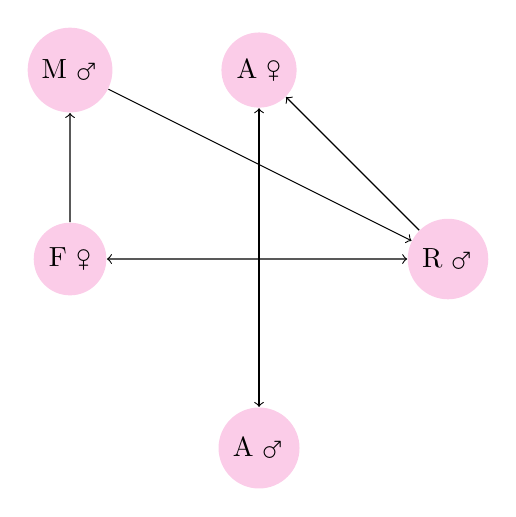
\begin{tikzpicture}
[scale=.8,auto=left,every node/.style={circle,fill=magenta!20}]
\node (Alexandre) at (0,0) {A \mars};
\node (Alexandrine) at (0,6) {A \venus};
\node (Robin) at (3,3) {R \mars};
\node (Floriane) at (-3,3) {F \venus};
\node (Miguel) at (-3,6) {M \mars};

\draw[<->] (Robin) to (Floriane);
\draw[<->] (Alexandre) to (Alexandrine);
\draw[->] (Robin) to (Alexandrine);
\draw[->] (Floriane) to (Miguel);
\draw[->] (Miguel) to (Robin);
\end{tikzpicture}



\end{document}
